%!TEX root = "../../../DA_GUI.tex"

%	--------------------------------------------------------
% 	Debugger: Popups
%	--------------------------------------------------------


\section{Popups}
\label{sec:deb-popup}
Im Debugger von C Compact gibt es mehrere Anwendungsfälle für Popup-Fenster. Popups werden verwendet, um weitere Informationen zu einem Array oder einem String in der Variablentabelle zu liefern und um Rückgabewerte von Funktionen zu visualisieren (dies ist allerdings optional, siehe auch \ref{sec:win-set}). Dabei handelt es sich im Prinzip um kleine Anzeigeflächen, die ein Swing-Element enthält (siehe Abbildung \ref{fig:popup-example}). Ein Popup wird ausgeblendet, sobald auf eine beliebige Fläche in einem Fenster von C Compact --- außerhalb des Popups --- geklickt wird.

\begin{figure}[htp]
\centering
\includegraphics[width=0.4\textwidth]{./media/images/gui/popup/popup-example.png}
\caption{Ein Popup zeigt den Rückgabewert einer Funktion.}
\label{fig:popup-example}
\end{figure}

\subsection{Initialisierung eines Popups}
Alle für das Popup relevanten Klassen befinden sich im Package \textbf{at.jku.ssw.cmm.gui.popup}. Die Popup-Funktionen selbst befinden sich in der Klasse \textbf{ImagePopup}. Zum Initialisieren werden aber die statischen Methoden in der Klasse \textbf{ComponentPopup} verwendet; diese Methoden übernehmen auch umständliche Positionsberechnungen für das Popup. Die Methode \textbf{createPopUp(...)} kann auch ohne das Parameter \glqq{}weight\grqq{} verwendet werden.
\begin{lstlisting}[language=JAVA]
public static void createPopUp( GUImain main, JComponent component, int x, int y, int w, int h, int orientation, double weight );
\end{lstlisting}

\begin{table}[h!]
\begin{tabular}{|ll|l|}
\hline 
GUImain & main  & Referenz auf das Hauptfenster, siehe \ref{sec:gui-main-impl} \\
\hline
JComponent & component & Das Swing-Element, das angezeigt werden soll \\
\hline
int & x & \multirow{2}{8cm}{Die Position, auf die das Popup zeigen soll} \\
int & y & \\
\hline 
int & w & \multirow{2}{8cm}{Höhe und Breite des Popups (Bezogen auf den äußeren Rand, \textbf{component} wird mit 5px Inset platziert)} \\
int & h & \\
\hline
int & orientation & Ausrichtung des Popups (siehe Unten) \\
\hline
double & weight [optional] & Position des Zeigers, Wert zwischen 0 und 1, Standard: 0.5\\
\hline
\end{tabular}
\caption{Parameter der Methode \textbf{createPopup(...)}}
\end{table}

\begin{figure}[h!]
\centering
\includegraphics[width=0.4\textwidth]{./media/images/gui/popup/popup-pos.png}
\caption{Positionierung eines Popups}\label{fig:deb-popup-pos}
\end{figure}

Der Parameter \textbf{orientation} legt fest, in welche Richtung das Popup zeigt. Das Popup hat immer einen Zeiger, der auf die mit \textbf{x} und \textbf{y} angegebene Position zeigt (siehe Abbildung \ref{fig:deb-popup-pos}). Für den Parameter \textbf{orientation} stehen vier Möglichkeiten zur Verfügung. Die Konstanten sind in der Klasse \textbf{ImagePopup} definiert:
\begin{itemize}
\item \textbf{NORTH:} Zeiger befindet sich am oberen Rand
\item \textbf{SOUTH:} Zeiger befindet sich am unteren Rand
\item \textbf{WEST:} Zeiger befindet sich am linken Rand
\item \textbf{EAST:} Zeiger befindet sich am rechten Rand
\end{itemize}

Mit dem Parameter \textbf{weight} kann die Position des Zeigers am Popup bestimmt werden. Der Wert 0 bedeutet, dass der Zeiger --- je nach Ausrichtung --- ganz links oder ganz oben ist. Wird dieser Parameter nicht angegeben, hat \textbf{weight} den Wert \textbf{0.5}.

\subsection{Implementierung}
Die Methoden zum Erstellen und Zeichnen des Popups befinden sich in der Klasse \textbf{ImagePopup}. Diese muss mit weniger praktischen Parametern initialisiert werden: mit x und y ist beispielsweise die linke obere Ecke des Popups anzugeben. Deshalb werden zum Initialisieren die statischen Methoden in der Klasse ComponentPopup verwendet. Diese rechnen die angegebenen Parameter auf die Popup-Positionen um.

\subsubsection*{Das Popup in das Hauptfenster zeichnen}
In Swing besteht jedes Fenster aus mehreren Schichten\footnote{https://docs.oracle.com/javase/tutorial/uiswing/components/rootpane.html}, die unterschiedliche Aufgaben übernehmen. Die oberste Schicht ist das sogenannte \textbf{GlassPane}. Dieses Panel ist standardmäßig deaktiviert. Wird es aktiviert, kann es verwendet werden, um über die Komponenten des Hauptfensters zu zeichnen und Events des Fensters abzufangen\footnote{https://docs.oracle.com/javase/tutorial/uiswing/components/rootpane.html\#glasspane}.

Die Klasse \textbf{ImagePopup(...)} erbt von \textbf{JPanel} und ist daher eine einfache Swing-Komponente. 

Mit der Methode \textbf{invokePopup(...)} wird eine beliebige Komponente zum GlassPane hinzugefügt und dort gezeichnet. Diese Methode befindet sich in der Klasse \textbf{GUImain} (siehe Kapitel \ref{sec:gui-main}), die das Hauptfenster von C Compact verwaltet.
\begin{lstlisting}[language=JAVA]
public void invokePopup(JPanel popup, int x, int y, int width, int height) {

	// Popup wird zum GlassPane hinzugefügt
	((JPanel) this.jFrame.getGlassPane()).add(popup);
	
	// Listener zum Schließen des Popuos wird initialisiert
	((JPanel) this.jFrame.getGlassPane()).addMouseListener(
		new PopupCloseListener(this.jFrame, ((JPanel) this.jFrame.getGlassPane()), popup, x, y, width, height));
		
	// GlassPane neu zeichnen
	((JPanel) this.jFrame.getGlassPane()).validate();
	((JPanel) this.jFrame.getGlassPane()).repaint();
}
\end{lstlisting}

In der Klasse \textbf{ImagePopup} wird die Methode \textbf{paintComponent}\footnote{http://www.oracle.com/technetwork/java/painting-140037.html\#callbacks} überschrieben. Dies ist eine der drei Methoden, die aufgerufen werden, wenn die Benutzeroberfläche neu gerendert werden muss. In gewisser Weise entspricht das der \textbf{paint}-Methode in ATW, allerdings spaltet Swing das Rendern auf drei unterschiedliche Methoden auf: \textbf{paintComponent} zeichnet das Element selbst, \textbf{paintBorder} zeichnet den Rand des Komponenten und \textbf{paintChildren} rendert die Komponenten innerhalb des zu zeichnenden Elementes. Durch diese Aufteilung können Manipulationen am Rendering eines Komponenten gezielter vorgenommen werden.

\begin{lstlisting}[language=JAVA]
@Override
public void paintComponent(Graphics g) {
        
    // Grenzen des Komponenten werden gesetzt
    switch( this.orientation ) {
    case NORTH:
    	g.setClip(g.getClipBounds().x, g.getClipBounds().y-10, g.getClipBounds().width, g.getClipBounds().height+10);
    	break;
    case SOUTH:
    	g.setClip(g.getClipBounds().x, g.getClipBounds().y, g.getClipBounds().width+10, g.getClipBounds().height+10);
    	break;
    case WEST:
    	g.setClip(g.getClipBounds().x-10, g.getClipBounds().y, g.getClipBounds().width+10, g.getClipBounds().height);
    	break;
    case EAST:
    	g.setClip(g.getClipBounds().x, g.getClipBounds().y, g.getClipBounds().width+10, g.getClipBounds().height);
    	break;
    }
    // Die Rendering-Methoden der Basisklasse werden aufgerufen
    super.paintComponent(g);
    super.paintBorder(g);
    	
    // Der Zeiger wird gezeichnet
    switch( this.orientation ) {
    case NORTH:
    	g.drawImage(image, centerX-10, centerY, image.getWidth(null), image.getHeight(null), this);
    	break;
    case SOUTH:
    	g.drawImage(image, centerX-10, centerY-15, image.getWidth(null), image.getHeight(null), this);
    	break;
    case WEST:
    	g.drawImage(image, centerX, centerY-10, image.getWidth(null), image.getHeight(null), this);
    	break;
    case EAST:
    	g.drawImage(image, centerX-15, centerY-10, image.getWidth(null), image.getHeight(null), this);
    	break;
    }
}
\end{lstlisting}

Mit der Methode \textbf{setClip} wird der Zeichenbereich des Popups so erweitert, dass der Zeiger gezeichnet werden kann, obwohl er außerhalb des JPanels liegt.

\subsubsection*{Popups mit Tabellen}
Um den Inhalt eines Arrays anschaulicher darzustellen, kann das Array in einem Popup geöffnet werden. Es wird dann als Tabelle dargestellt.

\begin{figure}[h!]
\centering
	\begin{minipage}{0.45\textwidth}
		\centering
		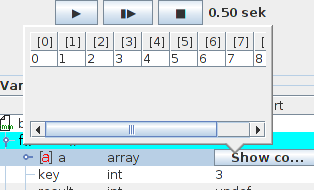
\includegraphics[width=1.0\textwidth]{./media/images/gui/popup/array1dim.png}
		\caption{Ein eindimensionales Array wird in einem Popup dargestellt}
		\label{fig:gui-popup-a1}
	\end{minipage}\hfill
	\begin{minipage}{0.46\textwidth}
		\centering
		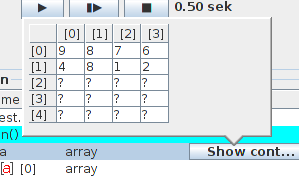
\includegraphics[width=1.0\textwidth]{./media/images/gui/popup/array2dim.png}
		\caption{Ein zweidimensionales Array wird in einem Popup dargestellt}
		\label{fig:gui-popup-a2}
	\end{minipage}
\end{figure}

Tabellen können grundsätzlich wie alle anderen Komponenten in einem Popup dargestellt werden. Für die Implementierung im Debugger (Abbildung \ref{fig:gui-popup-a1} und Abbildung \ref{fig:gui-popup-a2}) wurden allerdings ein eigenes Datenmodell und ein eigener Renderer erstellt. \textbf{TablePopupModel} ist ein Datenmodell, das den Inhalt eines Arrays korrekt darstellen kann. Für zweidimensionale Arrays wird die erste Tabellenspalte mit \textbf{TablePopupRenderer} gezeichnet, sodass sie wie die Kopfspalte der Tabelle aussieht (Abbildung \ref{fig:gui-popup-a2}).

